\documentclass{article}
\usepackage{mainPoly}

\title{Fonctions exponentielles}
\author{Terminale STMG2}
\date{}

\begin{document}
\maketitle
\section{Définition de l'exponentielle de base $a$}
\begin{tcolorbox}
On représente ci-contre les valeurs de la suite géométrique $(u_n)_{n \in \N}$ définie par $u_n = a^n$, avec $a > 0$.
\end{tcolorbox}
\begin{center}
\includegraphics[width=\textwidth]{Suite_geometrique.png}
\end{center}
\begin{tcolorbox}
\begin{definition}
Le prolongement aux réels de la suite $u_n$ est appelée \textbf{fonction exponentielle de base $a$}. Pour tout $x$ réel, l'image de $x$ par cette fonction est notée $a^x$. En particulier, si $x < 0$, alors cette image est définie par:
\begin{equation*}
a^x = \dfrac{1}{a^{-x}}
\end{equation*}
\end{definition}    
\end{tcolorbox}
\begin{example}
À l'aide d'une calculatrice, donner la valeur des image de fonctions exponentielles suivantes :
\begin{enumquestions}
\item $2^{3,5} = $\answersline
\item $10,2^{0,2} = $\answersline
\item $0,6^{-5,4} = $\answersline
\end{enumquestions}
\end{example}
\newpage
\section{Représentation graphique}
On représente ci-dessous la courbe représentative d'une fonction exponentielle de base $a$. Elle correspond au prolongement des points de coordonnées $(n;a^n)$.
\vspace*{0.5cm}
\begin{center}
\begin{minipage}{0.45\textwidth}
\includegraphics[width=\textwidth]{Fonction_exponentielle.png}
\end{minipage}
\begin{minipage}{0.45\textwidth}
\includegraphics[width=\textwidth]{Fonction_exponentielle_2.png}
\end{minipage}
\end{center}
\section{Sens de variation}
\begin{tcolorbox}
\begin{proposition}
Soit $a > 0$ un nombre réel. Alors,
\begin{itemize}
\item La fonction exponentielle de base $a$ est strictement croissante si et seulement si $a > 1$. 
\item La fonction exponentielle de base $a$ est strictement décroissante si et seulement si $a < 1$. 
\item La fonction exponentielle de base $a$ est constante si et seulement si $a = 1$. 
\end{itemize}
\end{proposition}
\end{tcolorbox}
\begin{center}
\includegraphics[width=\textwidth]{Variation_exponentielle.png}
\end{center}
\begin{example}
\hfill
\begin{enumquestions}
\item Comparer $3,4^{12}$ et $3,4^{15}$ : \answersline
\item Comparer $0,7^{3}$ et $0,7^{9}$ : \answersline
\end{enumquestions}
\end{example}
\begin{tcolorbox}
\begin{proposition}
Soit une fonction de la forme $f : x \mapsto k a^x$ avec $k$ un nombre réel et $a > 0$, alors le sens de variation de $f$ est donné grâce au tableau suivant.
\begin{center}
\begin{tabular}{|c|c|c|}
\hline
&$a > 1$&$a < 1$\\
\hline
$k > 0$& Croissante & Décroissante\\
\hline
$k < 0$& Décroissante & Croissante\\
\hline
\end{tabular}
\end{center}
\end{proposition}
\end{tcolorbox}
\newpage
\section{Propriétés algébrique de la fonction exponentielle}
\begin{tcolorbox}
\begin{proposition}
Soit $a$ un réel positif, ainsi que $x,y$ deux réels quelconques. Alors,
\begin{itemize}
\item $a^{x+y}=a^x \times a^y$
\item $a^{x \times y} = (a^x)^y$
\item $a^{x - y} = \dfrac{a^x}{a^y}$
\item $a^{-x} = \dfrac{1}{a^x}$
\item $a^{1/n} = \sqrt[n]{a}$
\item $a^0 = 1$
\end{itemize}
\end{proposition}
\end{tcolorbox}
\begin{example}
Simplifier les expressions suivantes en une puissance de $2$ :
\begin{enumquestions}
\begin{minipage}{0.45\textwidth}
\item $2^15 \times 2^12 = $ \answersline
\item $2^-7 =$ \answersline 
\item $(2^12)^{-5} =$ \answersline
\end{minipage}
\hfill
\begin{minipage}{0.45\textwidth}
\item $\dfrac{2^18}{2^5} = $ \answersline
\item $64^{4} =$ \answersline 
\item $2^4 + 2^4 =$ \answersline
\end{minipage}
\end{enumquestions}
\end{example}
\section{Cas particulier : taux d'évolution moyen}
\begin{definition}
On suppose qu'une quantité évolue de $T\%$ en $n$ étapes. Alors, si le coefficient multiplicateur de $T$ est noté $CM$, on dit que le \textbf{taux d'évolution moyen} est donné par le taux d'évolution $t$ dont le coefficient multiplicateur $cm$ est donné par
\begin{equation*}
cm = CM^{1/n}
\end{equation*}

Cela correspond au taux d'évolution constant associé à une étape. 
\end{definition}
\begin{center}
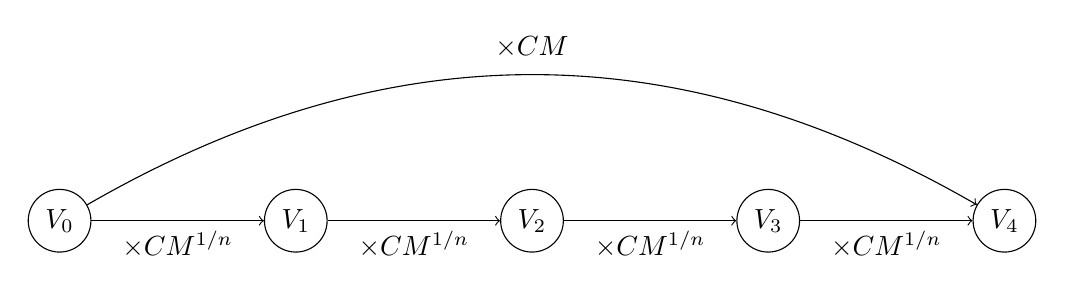
\begin{tikzpicture}
\node[draw,circle] (V0) at (0,0) {$V_0$};
\node[draw,circle] (V1) at (3,0) {$V_1$};
\node[draw,circle] (V2) at (6,0) {$V_2$};
\node[draw,circle] (V3) at (9,0) {$V_3$};
\node[draw,circle] (V4) at (12,0) {$V_4$};
\draw[->] (V0) -- (V1) node[midway,below] {$\times CM^{1/n}$};
\draw[->] (V1) -- (V2) node[midway,below] {$\times CM^{1/n}$};
\draw[->] (V2) -- (V3) node[midway,below] {$\times CM^{1/n}$};
\draw[->] (V3) -- (V4) node[midway,below] {$\times CM^{1/n}$};
\draw[->] (V0) to[bend left] (V4);
\draw (6,2.2) node {$\times CM$};
\end{tikzpicture}
\end{center}
\begin{example}
Le prix du loyer augmente de $54\%$ en quatre ans. Donner le taux d'évolution moyen de cette augmentation.

\begin{enumquestions}
\item On calcule d'abord le coefficient multiplicateur de $+ 54\%$ : $CM = $ \answersline
\item On calcule ensuite $cm = CM^{1/4} = $ \answersline
\item On déduit le taux d'évolution moyen $t = cm - 1 =$ \answersline
\end{enumquestions}
\end{example}
\end{document}